\chapter{System Design}
\label{ch:system-design}
\graphicspath{{./img/system-design/}}

In this section the block level system design is done and the direction finding algorithm decided on.
The design is done based on the user requirements specified in \Cref{ch:introduction} as well as the data and background gathered in \Cref{ch:lit-review}.
Once the system is designed, some simulations are run to show whether the algorithm performs as expected and also to highlight potential problems that need to be tackled.

\section{Sub-systems}
The DF system will consist of the following sub-systems.
A block diagram view of what's been described here is shown in \Cref{fig:system-design:signal-flow} with some additional requirements noted.

\subsection{Antenna Array}
The antenna array will receive the RFI signals. The user requirements state that a \SI{360}{\degree} field of view is necessary. Hence, a circular array will be used. The arrays needs to be useful in direction finding both narrow band and impulsive signals. This implies that a trade-off will have to be made in terms of element spacing when designing the array. If the element spacing is too large, the array will experience high amounts of phase ambiguity and perform poorly at narrow band DF. If the element spacing is too small the time difference for impulsive signals will be difficult to measure. The elements should be non-dispersive to facilitate keeping the structure of the impulsive signals. The number of elements to be used in the array will be explored later.

\subsection{Front End}
The front end will contain anti-aliasing filters and low noise amplifiers. For this project, a simple front end will be used. There will be no mixing or switching: the base band signal will be low pass filtered and amplified. The specifications of the filters and amplifiers will be specified based on the operating frequency band of the array and the sampling frequency of the ADCs. There will need to be an independent, identical RF chain for each element of the array.

\subsection{ROACH}
The ROACH board will have the main functions of doing analogue to digital conversion and the high-speed digital signal processing. The ROACH consists of a Virtex 5 FPGA and multiple ADC cards allowing all of the RF inputs will be digitsed independently. The purpose of the ROACH is to do real-time processing on the raw ADC samples, hence reducing the data rate to only signals of interest which can be sent to the computer and processed there.

\subsection{Computer}
The computer will receive input from the ROACH and do further DSP. Specifically, the final angle of arrival estimation. The computer needs to be able to log all of the data for future analysis and display the results of the direction finding to the user real-time in the field.


\begin{landscape}
  \thispagestyle{empty}
  \begin{figure}
    \centering
    \makebox[\textwidth][c] {
      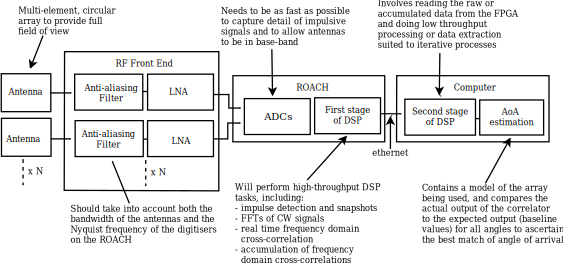
\includegraphics[width=\paperwidth, clip=true, trim = 80 500 80 80]{basic-flow}
      % left, bottom, right, top
    }
  \caption{Block diagram view of the flow of signals through the proposed direction finding system. The key function of the blocks has been noted on the diagram. }
  \label{fig:system-design:signal-flow}
  \end{figure}
\end{landscape}

\section{Direction Finding Algorithms}
With the above blocks available, this section goes into selecting an appropriate direction finding algorithm which meets the user requirements and refining what will be done in the first and second stage of DSP. Some additional requirements for the other blocks that arise from the selected algorithm are noted. 

This section details how the selected finding algorithm will be implemented on the system. Following will be a simulation of the algorithm and the system in operation is written in python and the output of this simulation is shown here, demonstrating that the algorithm is capable of carrying out the task.\\

There are two cases that the algorithm needs to deal with: weak narrow band signals and strong impulsive ones. The narrow band case naturally lends itself to frequency domain analysis, since the information about narrow band continuous signals is easily expressed in the frequency domain. The impulsive signals, however, are more naturally dealt with in the time domain as they are clearly bounded in time, existing only for a short duration, while being spread all over the frequency domain. 

As such, the selected algorithm contains two distinct parts: a phase interferometry component designed to direction find weak (below the noise floor) narrow band signals, and time difference of arrival part designed to locate strong (noticeable when plotted) short duration impulsive RFI.

\subsection{Phase Interferometry}
Phase Interferometry direction finding of narrow band signals will be done by phase comparison of the signal of interest as seen by each antenna in the array. The technique of phase interferometry has been extensively explored in the literature review.
\begin{enumerate}
  \item Steam the output of each ADC into a real-time FFT which is capable of producing Fourier transforms of the observed signals as fast as they are captured. The ADC inputs need to be fed into each FFT exactly in phase so that the output of each FFT can be meaningfully compared.
  \item Do a cross correlation between each pair of antennas (baseline). In the discrete frequency domain this means multiplying the value of each frequency channel from one antenna by the complex conjugate of the value of the corresponding frequency channels from another antenna. The output of this complex conjugate multiplication is a spectrum where the phase of each channel is the phase difference of the two input spectra. The amplitude of the channel is simply the product of the two input amplitudes, but it's not that important for this application.
  \item For weak signals, the phase of the cross correlation spectum may be dominated by noise. Assuming we've got Gaussian white noise, the noise component should average to zero. Taking advantage of this, we can add multiple of these spectra together. The signal component (phase difference of a baseline) will sum coherently while the noise component will sum to zero. As such, the more spectra are summed, the more the signal component will stand out of the noise.
  \item After sufficient spectra have been summed, save a result and extract the phase from each baseline spectra. Construct a \(N\)-dimensional vector of these observed baseline frequency differences,e where \(N\) is the number of baselines.
  \item Construct a \(N \times M\) matrix where each column of the matrix is a vector of theoretical baseline time differences for the AoA corresponding to that column. Here \(M\) is the number of angles which a simulation is taken for. It can be made as large as one wishes. A larger \(M\) means a higher resolution AoA estimation at the cost of more computational complexity.
  \item Calculate the RMS error between the observed vector and each column of the matrix. The column with the lowest RMS error is selected as the AoA of the signal. A measure of confidence can be given from the error.
\end{enumerate}

\subsection{Time Domain Direction Finding}
This technique is remarkably similar to the phase interferometry technique in that we are still measuring a parameter of the received signal from the array, comparing it to the theoretical response from the array at every angle and finding the angle whose expected output most closely matches the measured signal. The difference is that instead of the parameter of interest being the phase difference of a frequency channel, the parameter of interest is the time difference of the signal at each antenna. The process is as follows.

\begin{enumerate}
  \item Continuously monitor the signals received by the array (or a representative element) and detect if an impulse is observed.
  \item Capture a snapshot of the impulse by storing the raw ADC samples. As with the phase interferometry technique, the snapshot must be captured with each ADC sample exactly in phase with the other ADC samples to preserve the relative time difference of the signal as seen by the array elements.
  \item Do a time domain cross correlation between each pair of antennas. The peak of the correlation output corresponds to the time difference. Well, more specifically to the ADC clock cycles difference, but this can is a known frequency and hence can trivially be mapped to time difference. This is the equivalent process of measuring the phase differences of an frequency channel.
  \item Construct a \(N\)-dimensional vector of these observed time differences of each baseline where \(N\) is the number of baselines. This is the time domain equivalent of the vector of phase differences.
  \item Construct a \(N \times M\) matrix where each column of the matrix is a vector of theoretical baseline time differences for the AoA corresponding to that column. Here \(M\) is the number of angles which a simulation is taken for. It can be made as large as one wishes. A larger \(M\) means a higher resolution AoA estimation at the cost of more computational complexity.
  \item Calculate the RMS error between the observed vector and each column of the matrix. The column with the lowest RMS error is selected as the AoA of the signal. A measure of confidence can be given from the error.
\end{enumerate}

For the impulsive signals which the time domain DF will be used for, there is not an issue of ambiguity as the signals are not periodic like continuous narrow band signals are. Instead, the issue is one of resolution. In order to get accurate time difference readings, a high time resolution snapshot of the signals must be taken. This means a fast ADC. The higher the time resolution of the signal, the more cross correlation points there are and the greater the accuracy of the time domain measurement.

Fortu

Ambiguity not really an issue.
Discuss upsampling. Show plots.

The first step is to get the received signals into the frequency domain. This requires high throughput, real-time Fourier transforms. Fortunately the ROACH is well suited to this, as FFTs are one of its main applications. The next step is phase comparison. Once in the frequency domain, phase comparison is a matter of subtracting the phase of one element from another for each pair of elements in use. As it is necessary to see below the noise floor, a single FFT and phase comparison is not sufficient. If only one were taken the result would be dominated by noise and produce an incorrect result. The solution here is to do accumulation. We can consider each phase different measurement to be a small real signal component plus a large random and evenly distributed component from the noise. By summing multiple of these phase difference readings many times, the signal component will add coherently while the noise component will average to zero. 

\section{Algorithm Simulations}
In preparation for the implementation of the final DF algorithms, the following python python packages were written: 
directionFinder-backend has the code for an AntennaArray class which builds an array model out Antenna objects and can the calculate and returning a vector of the antenna array manifold. The phase-ambiguity package has logic for creating an AntennaArray object and then correlating the manifold vector from a reference direction to manifold vectors from all directions to find mathces and plot the results.

Parameters:
frequency range, number of frequency points, angle range, number of angle points, reference angle.

This produces a 3-d plot. Typically the 3-d plot is flattened to a 2-D image with colour used for the third dimension, rather than rendinging a 3-d image. The type of data being plotted naturally lends itself to a colour plot view.


Ideally we would like 4 dimensional vectors: frequency, reference angle, aoa, correlation. However, this is difficult to do. Hence, two simulation strategies are used: either fix reference angle and vary frequency and aoa. Or fix frequency and vary reference and aoa. They produce results with a different view: one shows the ambiguity perforamcne and a certain frequency, the other view shows the slice of the ambiguity performance over the whole frequency range. Process:

\begin{enumerate}
  \item A configuration file specifying how an antenna array is positioned in read in an an AntennaArray object is created.
  \item For each frequency bin in the frequency range:
  \begin{enumerate}
    \item The array manifold is generated for a reference \gls{aoa}. Default: \SI{0}{\degree}.
    \item For each angle in the incident angle range:
    \begin{enumerate}
      \item Calculate manifold.
      \item Correlate.
      \item Now have data point: frequency, incident angle, correlation between reference and this.
    \end{enumerate}
  \end{enumerate}
  \item plot all data points
\end{enumerate}

How about: vary reference and aoa and then pick the worst and plot that. Or average?? What's most interesting. Worst. Let's see worst case performance. 

\section{Frequency Domain Direction Finding}
How it works. Get phase difference between visibilities. 
Discuss algorithms. 

\subsection{Ambiguity Simulations}
Various ambiguity plots. 
Also show cross section for signal at 250 MHz
\begin{figure}
  \centering
  \begin{subfigure}{\textwidth}
    \centering
    \includegraphics[width=\textwidth, clip=true, trim = 0 15 53 0]{ambiguity03}
    % left, bottom, right, top
  \end{subfigure}\\[1em]
  \begin{subfigure}{\textwidth}
    \centering
    \includegraphics[width=\textwidth, clip=true, trim = 0 15 53 0]{ambiguity04}
  \end{subfigure}\\[1em]
  \begin{subfigure}{\textwidth}
    \centering
    \includegraphics[width=\textwidth, clip=true, trim = 0 15 53 0]{ambiguity05}
  \end{subfigure}
  \caption{Ambiguity plots for various antenna array sizes with reference signal arriving at \SI{0}{\degree}.}
\end{figure}
\begin{figure}
  \ContinuedFloat
  \centering
  \begin{subfigure}{\textwidth}
    \centering
    \includegraphics[width=\textwidth, clip=true, trim = 0 15 53 0]{ambiguity06}
    % left, bottom, right, top
  \end{subfigure}\\[1em]
  \begin{subfigure}{\textwidth}
    \centering
    \includegraphics[width=\textwidth, clip=true, trim = 0 15 53 0]{ambiguity07}
  \end{subfigure}\\[1em]
  \begin{subfigure}{\textwidth}
    \centering
    \includegraphics[width=\textwidth, clip=true, trim = 0 15 53 0]{ambiguity09}
  \end{subfigure}
  \caption{(cont'd) Ambiguity plots for various antenna array sizes with reference signal arriving at \SI{0}{\degree}.}
\end{figure}

\subsection{Accuracy Simulations}
RMS phase error vs RMS angular error.
\begin{figure}
  \centering
  \includegraphics[width=0.9\textwidth]{visibility-error-vs-df-error}
  \caption{This is a graphic showing some stuff}
\end{figure}

Again, simulation:
SNR vs number of correct correlation peaks.
Table: 
For an SNR: Do 1000 different cross correlations.RMS error in number of samples.
Do SNR: 10, 5, 2, 1, 0.5, 0.2, 0.1
